\documentclass[conference]{IEEEtran}
\IEEEoverridecommandlockouts

\usepackage{cite}
\usepackage{amsmath,amssymb,amsfonts}
\usepackage{algorithmic}
\usepackage{graphicx}
\usepackage{textcomp}
\usepackage{xcolor}
\usepackage{booktabs}
\usepackage{float}
\usepackage{multicol}
\usepackage{stfloats}
\usepackage{tikz}
\usetikzlibrary{shapes.geometric, arrows.meta, positioning}
\usepackage{url}
\def\BibTeX{{\rm B\kern-.05em{\sc i\kern-.025em b}\kern-.08em
    T\kern-.1667em\lower.7ex\hbox{E}\kern-.125emX}}

\begin{document}

\title{Multi-Domain Data Lakehouse: 
A Lightweight Lakehouse Strategy}

\author{
\IEEEauthorblockN{Arvesh Gosine\IEEEauthorrefmark{1},
Nie-l Constance\IEEEauthorrefmark{1}}
\IEEEauthorblockA{\IEEEauthorrefmark{1}Department of Computing and Information Technology\\
The University of the West Indies, St.\ Augustine Campus\\
Email: \{arvesh.gosine, niel.constance\}@my.uwi.edu}
}

\maketitle

\begin{abstract}
Many Modern Data Lakehouse solutions are proprietary, built for large Distributed Systems or are unaffordable to small teams. We have built a lightweight Lakehouse solution for such teams which focuses on the NYC Taxi and Limousine Commission dataset along with the National Oceanic and Atmospheric Administration Global Surface Summary of the Day dataset. Data is ingested, cleaned \& transformed and finally aggregated through an end-to-end pipeline using the Medallion Architecture with data validation checks built at the bronze and silver layer. We achieved this through local storage with MinIO buckets, a DuckDB query engine, dbt, Great Expectations, Delta Lake, Pyarrow and Apache Airflow. Aggregated data was then visualized using a Superset dashboard with a Trino query engine.  
\end{abstract}

\begin{IEEEkeywords}
Data Lakehouse, Distributed Systems Medallion Architecture, MinIO, DuckDb, dbt, Great Expectations, Delta Lake, Apache Airflow, Trino, Superset
\end{IEEEkeywords}

\section{Introduction and Problem Statement}
\label{sec:intro}

Most modern Data Lakehouse solutions use architectures suited for Distributed Systems which many small teams cannot afford. Small teams also do not require a large distributed system for their data pipeline as they only have one node available for processing. Furthermore, such solutions are proprietary and not readily available to small teams looking for lightweight solutions that are free. Such teams also have unreliable data pipelines which lack validation where schema drift occurs over time making the pipeline hard to maintain from one end to the other. Without a clear structure to the data processing and storage pipeline, organizations end up with unreliable data storage which cannot be audited or reliably used.

We devised an architecture using lightweight, open-source tools following the Medallion Architecture pattern, deployed entirely on a single node using MinIO as local cloud object storage. A supporting dashboard to visualize business ready data from this was also developed to prove that the data outputted from the full pipeline was valuable.

The TLC Yellow Taxi Trip and NOAA GSOD datasets were then chosen for this Lakehouse to be built around with a separate pipeline being developed for each. Both datasets are optimal for demonstrating this solution as they contain large amounts of data needing validation and further structuring to be truly useful to an organization with an end-to-end Medallion pipeline with validations being suitable for doing so. Both datasets also underwent schema evolution throughout the years which our solution intends to solve.

This matters because (i) both datasets exceed what single-machine tools like pandas handle comfortably, making a structured pipeline necessary, (ii) production Lakehouse tooling such as Databricks is cost-prohibitive for small teams, leaving a gap for open-source single-node alternatives, and (iii) both datasets exhibit real schema evolution over their publication history, making them genuine test cases for the pipeline's schema handling.

\section{Data Description and Source}
\label{sec:data}

\subsection{NYC Taxi and Limousine Commission (TLC) Yellow Trip Record Data\cite{tlc}}
    
The NYC TLC Yellow Taxi Trip Dataset is a publicly released archive
of every metered trip in New York City with metrics being given on trip distance, fare amount, pickup times, etc. Our Lakehouse pipeline ingests from 2019 onward with there being approximately 600+M records available for ingestion. 

The data is stored as parquet files with one file representing data for one month. There is approximately 2-6M records on average per month from 2019 onward with the year of 2019 have a noticeable high of 7+M records. Per file there are about 18-20 unique columns each of different data types and data ranges.

However, there are many issues present in the data such as there being negative values for column representing trip distances or fares, values of 0 for trip distances, invalid zone IDs or pickup times that are after dropoff times. Furthermore there are many nulls present in the data and column type changes that have occurred on ID columns. Notably there is also the addition of new columns such as the airport\_fee column from 2022 on ward.

\subsection{National Oceanic and Atmospheric Administration Global Surface Summary of The Day Dataset\cite{noaa}}

The NOAA Global Surface Summary of the Day (GSOD) Dataset is a publicly released archive of daily surface weather observations sourced from weather stations across the globe, with metrics being given on temperature, wind speed, precipitation, visibility, and atmospheric pressure, among others. Our Lakehouse pipeline ingests from 2019 onward with there being approximately 32+M records available for ingestion.

The data is stored as a collection of CSV files with a CSV file being generated for each station, the CSV files are then compressed into a tar.gz files and have files stored per year. One file has approximately 3-6M records and about 20-25 columns.

Given that many of the instruments used to record data are prone to error, many values in the dataset are invalid or contain sentinel values for bad measurements. Furthermore columns are sometimes missing across the dataset or contain conflicting datatypes which must be normalized.

\subsection{Data Cleaning}

There are approximately 100-300k faulty records per TLC Yellow Trip parquet file and 1-2.5M per NOAA GSOD file. The data is cleaned in our pipeline by removing records with nulls in important columns such as trip distance and pickup time, removing invalid values in important columns and by casting data types to a more correct and optimized type.

\subsection{Auxillary Data}
To make the TLC Yellow Trip dataset truly useful, it was joined on the TLC Taxi Zone Lookup table to get the name of pickup and dropoff locations.


\section{Literature Review}
\label{sec:lit}

Data lakehouse architecture has emerged as the dominant paradigm for 
organizations seeking to unify the scalability of data lakes with the 
reliability guarantees of traditional data warehouses. Armbrust et al.\ 
\cite{armbrust2021lakehouse} formally introduced the lakehouse concept, 
arguing that open direct-access formats such as Apache Parquet, combined 
with a metadata and transaction layer, could deliver warehouse-grade 
performance and ACID compliance directly over object storage. The same 
group's earlier work on Delta Lake \cite{armbrust2020deltalake} 
demonstrated that a transaction log stored alongside the data files 
enables snapshot isolation, schema enforcement, and time travel at scale, 
all without a separate catalog service. Our pipeline adopts this approach 
directly, using \texttt{delta-rs}, the Rust-native implementation of the 
Delta Lake protocol, to write and manage Delta tables in MinIO across all 
three medallion layers.

The medallion architecture pattern itself---organizing a lakehouse into 
progressive Bronze, Silver, and Gold layers---was coined and popularized 
by Databricks as a practical organizing principle for the lakehouse 
paradigm \cite{databricks_medallion}. Bronze captures raw, immutable 
data with minimal transformation; Silver applies cleaning, validation, 
and type normalization; Gold contains business-level aggregations ready 
for analytical consumption. This layered approach decouples ingestion 
from curation, allows reprocessing from source without re-extracting 
upstream data, and provides a shared vocabulary for engineering and 
analytical teams. Our pipeline follows this pattern faithfully, with 
data quality gates inserted between Bronze and Silver and between Silver 
and Gold to prevent bad data from propagating downstream.

For the transformation layer, we chose DuckDB \cite{raasveldt2019duckdb} 
over distributed systems such as Apache Spark. Raasveldt and Mühleisen 
introduced DuckDB as an embeddable analytical database designed to 
execute OLAP queries efficiently within a single process, without the 
overhead of a distributed scheduler or cluster manager. Benchmarked 
against systems such as HyPer and MonetDBLite on TPC-H workloads, DuckDB 
demonstrated competitive analytical performance on commodity hardware 
through its vectorized columnar execution model. For our dataset volumes 
--- on the order of hundreds of millions of rows per year when fully 
ingested --- a single-node DuckDB instance provides sufficient throughput 
while eliminating the operational complexity, memory tuning, and startup 
overhead that characterize Spark deployments. This choice is a deliberate 
architectural decision in favour of simplicity and accessibility for 
small teams.

Data quality validation is a recognized first-class concern in production 
data pipelines. Great Expectations \cite{ge_docs} provides an open-source 
Python framework for defining, executing, and documenting data quality 
checks as declarative \emph{Expectations} --- assertions about what valid 
data should look like. Checkpoints bundle Expectations into validation 
runs that can be triggered by an orchestrator and configured to emit 
alerts on failure. This approach has been characterized as unit testing 
for data: it separates the specification of quality from the pipeline 
logic itself, making quality requirements explicit and auditable. We 
apply Great Expectations checkpoints after Bronze ingestion and after 
Silver transformation, using the validation results to gate downstream 
processing and to generate persistent data quality reports.

Pipeline orchestration is handled by Apache Airflow \cite{airflow_docs}, 
which was originally developed at Airbnb in 2014 to manage the 
complexity of growing data pipelines and open-sourced in 2015 before 
graduating to a top-level Apache Software Foundation project. Airflow 
represents workflows as directed acyclic graphs (DAGs) of tasks, 
enabling dependency-aware scheduling, automatic retries on failure, and 
a web interface for monitoring pipeline state. Its Python-native DAG 
authoring model makes it straightforward to encode conditional logic --- 
for example, halting downstream tasks when a Great Expectations checkpoint 
fails --- which is central to the quality-gated design of our pipeline.

Gold-layer aggregations are managed using dbt (Data Build Tool) 
\cite{dbt_docs}, an open-source analytics engineering framework that 
allows transformations to be expressed as SQL \texttt{SELECT} statements 
organized into a dependency graph. dbt handles materialization, 
dependency resolution, and incremental model execution, and brings 
software engineering practices such as version control, modular 
composition, and built-in testing to the SQL transformation layer. 
Originally released in 2016, dbt has become a standard in the modern 
data stack for managing the T in ELT workflows. In our pipeline, dbt 
models are exposed over a lightweight FastAPI service so that Airflow 
can trigger Gold-layer builds via HTTP without requiring a shared 
execution environment.

Our overall approach is closest in spirit to small-team lakehouse 
implementations that prioritize operational simplicity over distributed 
scale. The body of literature on production data engineering 
\cite{armbrust2021lakehouse, armbrust2020deltalake} consistently 
identifies schema drift, lack of data lineage, and the absence of 
validation as the primary failure modes in data lake deployments at 
scale. Our pipeline addresses all three directly: Delta Lake's 
transaction log provides lineage and time travel; the explicit 
Bronze-Silver-Gold schema normalization step resolves the column 
renaming and type inconsistencies present in both source datasets; and 
Great Expectations checkpoints enforce validation contracts at every 
layer boundary. Rather than reaching for a graph neural network or a 
distributed compute cluster, we demonstrate that these failure modes 
can be addressed with lightweight, composable, open-source tooling 
sized for a single node.

%% Architecture Diagram
\begin{figure*}[b]
    \centering
    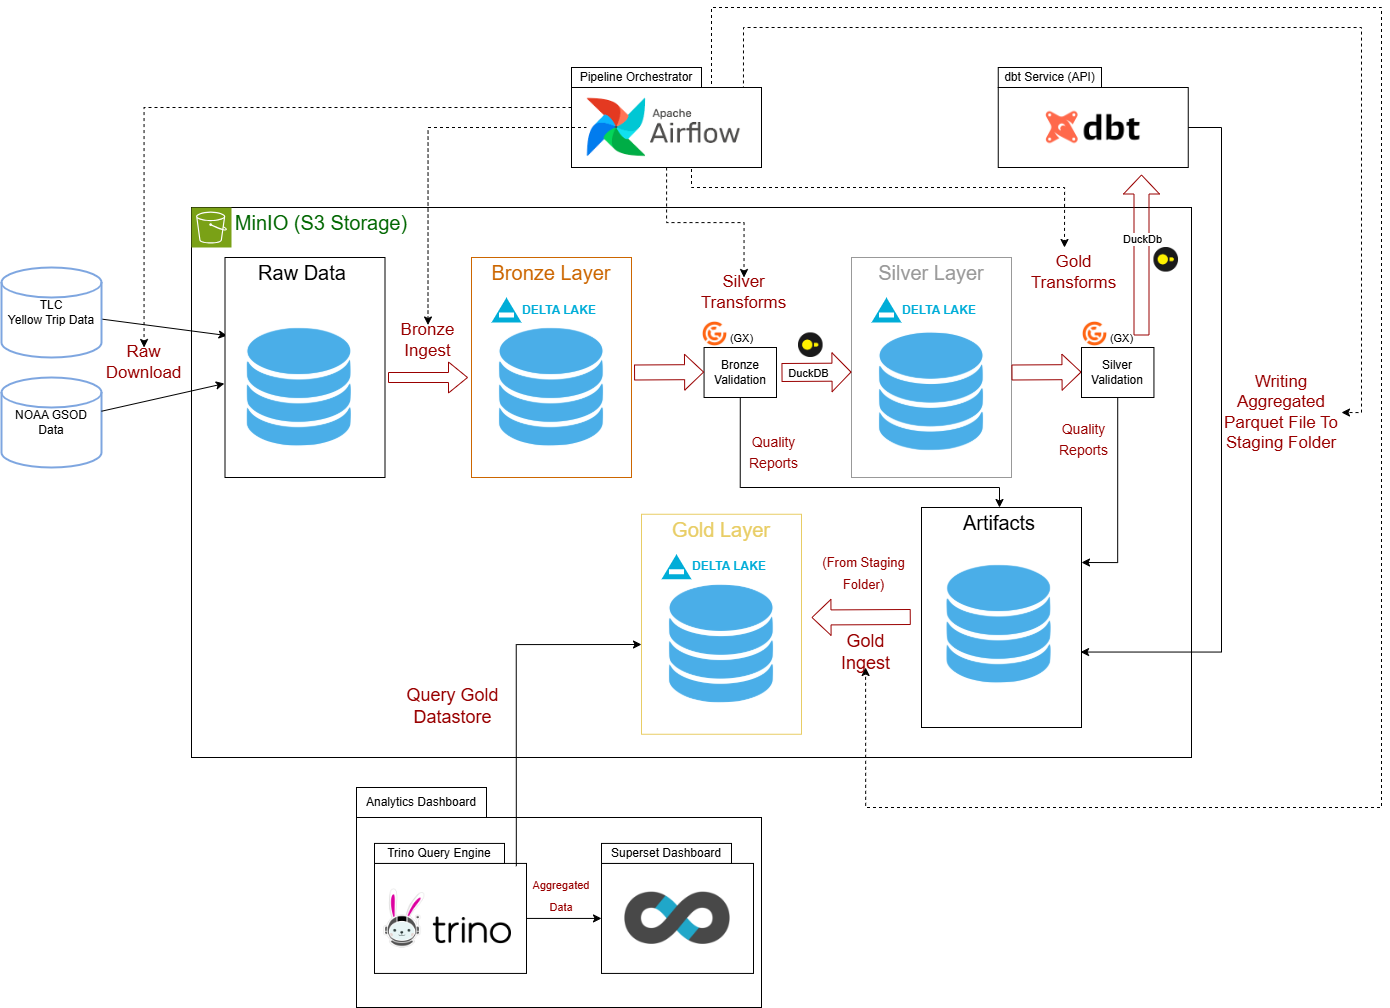
\includegraphics[width=\textwidth]{Architecture Diagram.drawio.png}
    \caption{Architecture diagram of Lakehouse}
    \label{fig:architecture}
\end{figure*}

\section{Methodology}
\label{sec:method}

\subsection{Architectural Overview}

\subsubsection{MinIO}
Figure~\ref{fig:architecture} displays the Lakehouse architecture built for this project. The storage service chosen for this design was MinIO \cite{minio_docs} which is a datastore similar to an AWS S3 datastore. MinIO provides us with local storage allowing us to completely bypass the cost of cloud storage platforms such as AWS S3 or Azure Blobs. Our design has a data bucket for the Bronze, Silver and Gold Layer storage but also includes a bucket for raw files downloaded and a bucket for Artifacts generated throughout the pipeline. It should also be noted that the Artifact bucket acts as a staging area for Gold Ingestion which we discuss later.

\subsubsection{Delta Lake}
Delta Lake \cite{armbrust2020deltalake} was then chosen to format all parquet files stored in our Bronze, Silver and Gold buckets. Within these buckets we only have parquet files stored as Delta Tables which allows for time travel queries, schema enforcement and ACID transactions. It should also be noted that Delta Tables stored here are partitioned on the year and month of when the data was recorded. Delta Tables also allows us to merge schemas in the event that new columns were added which helps address our problem of schema evolution.

\subsubsection{Great Expectations}
Great Expectations \cite{ge_docs} was used to create validation suites at both the Bronze and Silver layer of the Lakehouse. If checks fail at any one of these validation check points we halt the flow of the pipeline for said month or year and move on to processing of another year or month. Furthermore Great Expectations provides us with alerting and reporting of our validations where reports generated are stored in the Artifacts bucket of MinIO. These reports inform us of which checks failed and which passed and can be used to audit the pipeline more efficiently.

\subsubsection{DuckDB}
DuckDB \cite{raasveldt2019duckdb} was chosen to act as our query engine for Silver cleaning \& transforms and Gold aggregations. DuckDB allows for processing of millions of records on a single node without the overhead of distributed systems or JVM used by Apache Spark. It acts as a lightweight in-process analytical database which runs in the same Python process as our processing scripts which allows. Furthermore it's vectorized columnar execution model allows for competitive OLAP performance against distributed engines on datasets of the scale processed in this pipeline.

\subsubsection{dbt}
dbt \cite{dbt_docs} then handles the management of our Gold layer aggregations by providing modular SQL statements whose dependency graph is resolved and executed automatically. This allows for a separation of concerns where transforms are kept separate from the orchestration layer entirely. The models generated here are reusable and version-controlled allowing for testing and documenting of each individual model. Furthermore dbt's model dependency graph ensures aggregations execute in the correct order without manual sequencing.

\subsubsection{FastAPI}
An lightweight API was also developed over the dbt project to expose it to our pipeline for orchestration without our pipeline needing to manually interact with it. Instead it is accessed through an HTTP request to run the desired aggregations. FastAPI \cite{fastapi_docs} was used for this to provide us with a quick and lightweight API to access dbt. This decoupling allows the dbt project to evolve separately from the rest of our pipeline.

\subsubsection{Apache Airflow}
The entire pipeline is then orchestrated with Apache Airflow \cite{airflow_docs} allowing for an automated execution of the pipeline with no manual inputs needed by representing the pipeline as a Directed Acyclic Graph (DAG). The pipeline can be correctly sequenced using Airflow with scheduled runs being set at preset dates. It also allows for back filling of previous runs from the current date. The web GUI of this also provides real time logging and visualization of the pipeline run. Furthermore Airflow enforces our validation gates with the pipeline halting for a scheduled run if the validation check fails at any one of its checks.

\subsubsection{Pyarrow}
Although not stated in the diagram, we also use Pyarrow \cite{pyarrow_docs} within the architecture for Delta Table reads and writes. This was due to a limitation of DuckDB not being able to execute Delta Table read and writes on its own due to conflicts with S3 credentials being sent to MinIO during reads and writes. This may have been due to a limitation with the version used for this project (1.4.4) with the rust kernel of delta-rs not communicating correctly with DuckDB. Beyond this Pyarrow also provided an in-memory columnar format for data processing that can compete with Spark which further helps in optimizing this system for a single node.

\subsubsection{Superset}
Superset \cite{superset_docs} was also used in this design to provide for dashboard visualizations of our Gold layer aggregations. It allowed for real time dashboard analytics with a built in SQL lab for further querying of the gold data and a simple to use GUI interface for quickly designing charts to visualize data.

\subsubsection{Trino}
Trino \cite{trino_docs} serves as the query engine for the analytical serving layer, sitting between MinIO and the Superset dashboards. Through its Delta Lake connector, Trino reads Gold Delta tables directly from MinIO without requiring data to be moved or copied into a separate analytical store, keeping the serving layer decoupled from the pipeline while still exposing data as standard SQL tables. This separation means Superset can issue familiar SQL queries against live Gold data through Trino without any knowledge of the underlying Delta format or object storage layout, closing the loop from raw ingestion to interactive dashboards entirely within the open-source stack.

\subsection{Pipeline overview}

%% Pipeline Image
\begin{figure}[h]
\centering
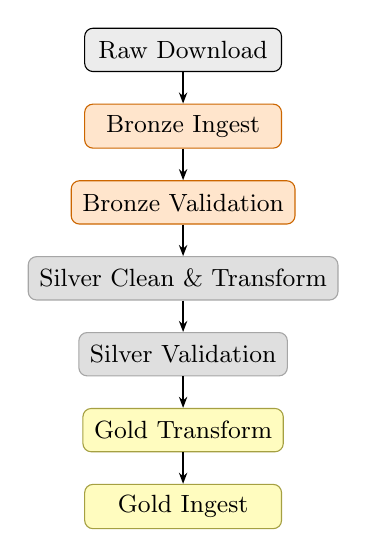
\begin{tikzpicture}[
    node distance = 0.4cm and 0.3cm,
    box/.style = {
        rectangle, rounded corners=3pt,
        minimum width=2.5cm, minimum height=0.55cm,
        font=\small, text centered,
        inner sep=4pt
    },
    raw/.style    = {box, draw=black,         fill=gray!15},
    bronze/.style = {box, draw=orange!80!black, fill=orange!20},
    silver/.style = {box, draw=gray!70,        fill=gray!25},
    gold/.style   = {box, draw=yellow!60!black, fill=yellow!25},
    arr/.style    = {-{Stealth[length=4pt]}, thick}
]

%% Column Nodes
\node[raw]    (dl)  {Raw Download};
\node[bronze, below=of dl]  (bi)  {Bronze Ingest};
\node[bronze, below=of bi]  (bv)  {Bronze Validation};
\node[silver, below=of bv]  (sc)  {Silver Clean \& Transform};
\node[silver, below=of sc]  (sv)  {Silver Validation};
\node[gold,   below=of sv]  (gt)  {Gold Transform};
\node[gold,   below=of gt]  (gi)  {Gold Ingest};

%% Arrows 
\draw[arr] (dl) -- (bi);
\draw[arr] (bi) -- (bv);
\draw[arr] (bv) --  (sc);
\draw[arr] (sc) -- (sv);
\draw[arr] (sv) -- (gt);
\draw[arr] (gt) -- (gi);

\end{tikzpicture}
\caption{End-to-end Medallion pipeline for datasets.}
\label{fig:pipeline}
\end{figure}

Figure~\ref{fig:pipeline} shows the end-to-end Medallion pipeline used to process the two datasets discussed earlier. The pipeline first begins with a raw download step to get the data programmatically from each source. Following this at the Bronze Layer we have a Bronze Ingest step which ingests our raw data into the Bronze bucket followed by a Bronze Validation step which ensures the data was ingested successfully and is suitable for the pipeline. At the Silver Layer there is a Silver Clean \& Transform step which cleans the data of any invalid records and transforms it by adding enriched columns and optimizing data types with the final result being stored in our Silver bucket. A Silver Validation is then done after ensuring the Silver Clean \& Transform was done successfully. Finally at the Gold Layer we aggregate the data into useful analytical tables at the Gold Transform Step and then ingest it into our Gold bucket at the Gold Ingest Step. 

\subsubsection{Raw Download}
At the raw download step data is programmatically downloaded from the source website and stored as its raw file type in the raw bucket of MinIO. The data is requested over an HTTP request with one file downloaded at a time. 

\subsubsection{Bronze Ingest}
The Bronze ingest step then has variations for its implementation for both datasets. Both variations involve fetching the raw file from the raw bucket of MinIO and adding source\_year, source\_month, ingested\_at and source\_file columns to the file for auditing which is done with Pyarrow. Both variations also involve writing the file as a Delta Table to the Bronze bucket of MinIO with it being partitioned on the source\_year and source\_month column. Furthermore the schemas of data is merged if during the Delta table write new columns are detected. 

However, there is variation in how the raw data files are prepared for Delta table writes, most notably with the NOAA GSOD dataset. The TLC Yellow Trip records are simply read into a Pyarrow table, have audit columns added and then written to the Bronze bucket following the method discussed earlier. The NOAA GSOD data must be extracted from the tar.gz file stored in MinIO first into a temp directory. The CSV files in this directory must then be merged into one large Pyarrow table with the table being indexed on the STATION\_ID column of the CSVs. Furthermore, the STATION\_ID column must be casted to a string for this work as the data type is often different per file. The usual auditing and Delta Table write to the Bronze bucket is then done after this.

\subsubsection{Bronze Validation}

Both datasets undergo Bronze validation using Great Expectations  immediately after Bronze ingestion and before any Silver transformation is permitted to run. The validation suite for each dataset is constructed fresh on each run to prevent stale suite definitions from persisting across executions, with any prior suite, batch definition, validation definition, and checkpoint being explicitly deleted before recreation. This ensures that re-runs of the pipeline for a given period always validate against the current suite definition rather than a cached version.

Both suites share the same three-rule structure. The first rule validates that the row count for the batch falls within an expected range, catching both truncated ingestion and unexpectedly large files that may indicate a data source anomaly. The second rule verifies that all expected columns are present in the Bronze table, including the four audit columns added during ingestion (ingested\_at, source\_file, source\_year, and source\_month)  ensuring the schema contract between Bronze and Silver is upheld which addresses schema evolution in terms of columns being removed. The third rule checks that critical columns do not exceed a 10\% null rate, guarding against data corruption or failed ingestion that may have produced a structurally valid but largely empty table.

There are however differences in the specific thresholds and columns validated between the two datasets reflecting their differing schemas and granularities. The TLC suite validates on a per-month basis with an expected row count between 200,000 and 6,000,000 rows, checking null rates across eight critical columns including pickup and dropoff datetimes, fare amount, and trip distance. The NOAA suite validates on a per-year basis given that GSOD data is ingested annually, with an expected row count between 1,000,000 and 5,000,000 rows and null checks applied across twelve meteorological columns including temperature, wind speed, precipitation, and visibility.

Upon completion of each batch validation, the checkpoint result is both printed to the console with a per-check breakdown of passed and failed expectations and saved as a JSON report to the Artifacts bucket in MinIO under a path structured by dataset and layer. If any check fails, the month or year is recorded as failed and the pipeline exits with a non-zero status code, which Airflow interprets as a task failure and uses to halt all downstream Silver tasks for that batch.

\subsubsection{Silver Cleaning \& Transforming}

The Silver transformation step reads from the Bronze Delta table for each batch, applies a multi-stage DuckDB SQL query in a single pass, and writes the cleaned and enriched result back to the Silver Delta table in MinIO. Both datasets follow the same structural approach --- a Bronze partition is read into a PyArrow table, registered with DuckDB as a virtual table, passed through the transformation query, and the resulting PyArrow table is written back to Silver via a predicate overwrite, ensuring only the specific year and month partition is replaced rather than the entire table.

The transformation query is structured in three stages for both datasets. The first stage filters out records that fail quality rules, dropping them entirely so that no bad data passes through to Silver. For the TLC dataset these rules enforce non-null values on eight critical columns, a valid fare\_amount between 0.0 and 500.0, a passenger\_count between 1 and 6, a trip duration between 1 and 1440 minutes, pickup before dropoff, and that the record belongs to the correct year and month partition being processed. For the NOAA dataset the rules enforce non-null values on eight critical columns, sentinel value removal where GSOD uses values such as 9999.9 and 999.9 to represent missing observations, geospatial validity bounds on LATITUDE, LONGITUDE, and ELEVATION, physical plausibility bounds on all weather metrics, cross-field consistency checks such as dew point never exceeding temperature and minimum temperature never exceeding maximum, and that the record belongs to the correct year.

The second stage applies explicit type casts to all retained columns for memory optimization. For the TLC dataset, passenger\_count and pickup\_hour are cast to UTINYINT, PULocationID and DOLocationID to USMALLINT, and trip\_distance and fare\_amount to FLOAT, reducing the per-row memory footprint compared to the default 64-bit types present in the Bronze table. For the NOAA dataset, all weather metrics are cast from their original string representations to FLOAT, station coordinates to FLOAT, and elevation to SMALLINT. These casts are applied inline within the SELECT list rather than as a separate processing step, keeping the transformation consolidated within a single query execution.

The third stage derives all enrichment columns added at the Silver layer. For the TLC dataset seven derived columns are added: trip\_duration\_minutes computed via DATEDIFF, trip\_speed\_mph computed as distance divided by duration in hours and set to null when duration is zero to avoid division errors, pickup\_hour extracted via HOUR, pickup\_day\_of\_week via DAYOFWEEK, payment\_method decoded from the numeric payment\_type via a CASE statement into human-readable labels, day\_name via DAYNAME, is\_weekend derived from the day of week, and pickup\_date extracted as a DATE. For the NOAA dataset fourteen derived columns are added including season\_northern assigned by month via CASE, day\_name and is\_weekend mirroring the TLC approach, temperature conversions from Fahrenheit to Celsius for TEMP, MAX, and MIN, wind speed conversions from knots to kilometres per hour for WDSP, MXSPD, and GUST, and four boolean weather event flags --- is\_freezing set when temperature is at or below 32\textdegree F, is\_extreme\_heat set when temperature is at or above 100\textdegree F, has\_precipitation set when PRCP is greater than zero, and is\_gale set when wind speed meets or exceeds 34 knots. Both datasets also add a processed\_at audit timestamp recording when the Silver transformation ran for each batch.

\subsubsection{Silver Validation}

Silver validation runs immediately after the Silver transformation for both datasets and before any Gold aggregation is permitted to execute. Like the Bronze suite, each Silver suite is rebuilt fresh on every run with prior definitions explicitly deleted to prevent stale state from persisting across executions. The Silver suites are considerably more comprehensive than their Bronze counterparts, reflecting the stricter quality guarantees that the Silver layer is expected to provide --- where Bronze validates structural integrity, Silver validates business rule compliance and the correctness of all derived columns produced during transformation.

Both suites share the same foundational rule structure but are expanded significantly beyond the three Bronze rules. The first rule again validates row count bounds, though the Silver thresholds are set slightly lower than Bronze to account for records dropped during cleaning. The second rule verifies the full Silver schema including all derived columns added during transformation --- for the TLC dataset this includes trip\_duration\_minutes, trip\_speed\_mph, pickup\_hour, etc, while the NOAA dataset adds meteorological derivations such as temp\_c, wdsp\_kmh, etc. The presence of these columns in Silver directly confirms that the transformation step executed its full logic rather than producing a partial result.

The null checks at Silver are split into two tiers. Critical columns --- those that the cleaning step explicitly enforced non-null values for ---  are checked at a 100\% non-null threshold, while legitimately sparse columns such as trip\_speed\_mph, which is null when trip duration is zero, and meteorological columns such as GUST and SNDP, which are not recorded at all stations, are checked at a 75\% non-null threshold. This two-tier approach avoids false failures on columns that are validly sparse while still catching unexpected null propagation in columns that should always be populated after cleaning.

A new value range check rule is then introduced to ensure cleaning of the data at the Silver layer was properly executed with there being no invalid values or unreasonable values being present for gold aggregations. This varies per dataset with the TLC dataset doing range checks on the fare\_amount, trip\_distance, passenger\_count, trip\_duration\_mins, pickup\_hour and pickup\_day\_of\_week columns. The NOAA GSOD dataset then has range checks on measurements for precipitation, temperature, wind speed and visibility columns done to ensure all measurements going foward are reasonable.

Categorical set checks validate all derived columns whose values are produced by CASE logic in the transformation SQL. For the TLC dataset, payment\_method must contain only the six defined payment categories, day\_name must be a valid day of the week, and is\_weekend must be boolean. For the NOAA dataset, season\_northern must be one of the four seasons, and all four weather event flags must be boolean. Any broken CASE statement in the transform would immediately surface here as a categorical violation.

The NOAA Silver suite includes two additional rules not present in the TLC suite, reflecting the nature of the NOAA data model with there being more unreliable data and measurements. A uniqueness check enforces that the compound key of STATION and DATE is unique across the table, ensuring no station has duplicate daily records after merging. A second check verifies that all twelve months are represented in the source\_month column for a given year, catching cases where a partial ingestion or failed month would silently produce an incomplete annual dataset that would then corrupt downstream Gold aggregations. As with Bronze, all results are printed to the console with a per check breakdown and saved as JSON reports to the Artifacts bucket in MinIO, with a non-zero exit code halting all downstream Gold tasks in Airflow if any check fails.

\subsubsection{Gold Transform}

The Gold Transform then runs after the Silver Validations are successful with a separate dbt project handling all aggregations with DuckDB being used as the query engine for it. dbt is interacted with via an API created using FastAPI with aggregations being triggered via a request over HTTP for the desired dataset and month for that dataset. This was done to decouple dbt from the overall pipeline and for Apache Airflow to be able to easily orchestrate this step with the rest of the pipeline.

Both datasets have staging models created where certain columns are renamed for readability such as tpep\_pickup\_datetime to pickup\_datetime in the TLC Yellow Trip dataset and the columns being converted to lowercase in the NOAA GSOD dataset. Due to DuckDB's limitation of not being able to read Delta Tables, the tables must be read as parquet files instead and filtered on source\_year and source\_month columns. It should also be noted that all Gold aggregations are done per month for each dataset in the pipeline.

The TLC Yellow Trip dataset also has the addition of an intermediate table in the dbt project where the pickup location id and drop off location id columns are joined on the TLC Taxi Zone Lookup to get the appropriate names of the locations. Furthermore the appropriate borough name is also added to this intermediate table. All gold models created then use this intermediate table for the TLC Yellow Trip dataset.

Gold models containing the aggregated business analytical data is then generated for both datasets. The TLC Yellow Trip dataset has 5 gold models created: a daily summary (weekday), hourly summary, individual day summary, zone performance summary and payment summary. The NOAA GSOD then has 3 gold models being a daily climate summary, monthly climate summary and station metrics. For all gold models, the data is aggregated and grouped by certain columns to provide summaries for the datasets ingested. 

Each of these gold models are then stored as individual parquet files to a staging area in the artifacts bucket of MinIO since DuckDB is unable to write Delta tables. Only one parquet file per model can live in this staging area at the time which results in only one month being able to be processed at a time in the pipeline. This method was chosen to save storage space in the artifact bucket, multiple files could live here at a time however as more files were processed the bucket would become overly large and impact performance.

\subsubsection{Gold Ingest}

The Gold Ingest then handles all Delta table writes to the Gold bucket of the Lakehouse by ingesting the parquet files generated from the Gold transform. Given that only one month can be processed at a time due to the staging area limitation, the Gold ingest only ingest one months worth of data for both datasets from the Gold aggregations.

To ingest the parquet files storing the aggregated data, we use Pyarrow to read the data into an arrow table which is then written as a Delta table to the Gold bucket. The table is also partitioned on source year and source month like the other layers with schemas being merged for any new columns added by the dbt project. However,removal of columns are not handled by the gold ingest as columns should not be removed from the existing dbt project. This is then done for each aggregated table for the dataset called by the API to be ingested for the specified month.

\subsection{Query Optimization}
To efficiently optimize queries we used methods such as partitioning the datasets on source year and source month columns for efficient retrieval. Along with this we also casted large data types to smaller ones to save memory within our storage buckets. The use of Pyarrow to read/write parquet files and delta tables also helps in optimizing performance throughout the application.

\section{Analysis and Results}
\label{sec:results}

\begin{table}[h]
    \centering
    \caption{Table showing row count at each layer for each dataset}
    \label{tab:rowcounts}
    \begin{tabular}{|l|c|c|c|}
        \hline
        \textbf{Dataset} & \textbf{Bronze Layer} & \textbf{Silver Layer}  & \textbf{Gold layer} \\
        \hline
        TLC Yellow Trip Data & 600M+ & 500M+ & 250K+ \\
        NOAA GSOD Data & 32M+ & 20M+ & 12M+ \\
        \hline
    \end{tabular}
\end{table}

\subsection{Headline results}
Table~\ref{tab:rowcounts} reports the number of rows ingested at each layer for both datasets. We see that the TLC Yellow Trip data has the most amount of rows with on average 100M rows being dropped from Bronze to Silver and only 250K useful rows being generated for Gold aggregated data. The NOAA GSOD data being smaller on the other hand only has 32M on average at the Bronze layer and ha 12M rows dropped after Silver cleaning and transformations. However the Gold layer for this dataset has 12M records with there being more data required to be present after aggregations for the dataset to be truly useful.

\subsection{Query Optimization Results}

\begin{table}[h]
    \centering
    \caption{Table showing speed up from partitioning on data read}
    \label{tab:partioning}
    \begin{tabular}{|l|c|}
        \hline
        \textbf{Baseline} & \textbf{Partitioned} \\
        \hline
        75.23s & 4.06s \\
        \hline
    \end{tabular}
\end{table}

\begin{table}[h]
    \centering
    \caption{Table showing memory saved from data type casting (TLC Yellow Trip Data)}
    \label{tab:datatype}
    \begin{tabular}{|l|c|}
        \hline
        \textbf{Baseline} & \textbf{Optimized} \\
        \hline
        60MiB & 53.85MiB \\
        \hline
    \end{tabular}
\end{table}

Table~\ref{tab:partioning} shows the speedup in reading data from both datasets with and without partitioning. The baseline shows the time taken to read data for a certain month and year with a normal WHERE filter using DuckDB while the partitioned time shows the same data read but by using the partitioned columns of source\_year and source\_month which is added to both datasets. This is an 18.52x speedup observed with partitioning which greatly helps in optimizing our lakehouse for a single node to run on.

Table~\ref{tab:datatype} shows the memory size decrease for the TLC Yellow Taxi Trip data after optimizing the data types of columns to smaller types which still preserve the original values of the data. We observe 6.85MiB of storage being saved per file on average after optimizing data types which would allow the Lakehouse to comfortably run on a single node without incurring high storage costs.

\subsection{Deliverables}

%% Taxi Dashboard Diagram
\begin{figure*}[t]
    \centering
    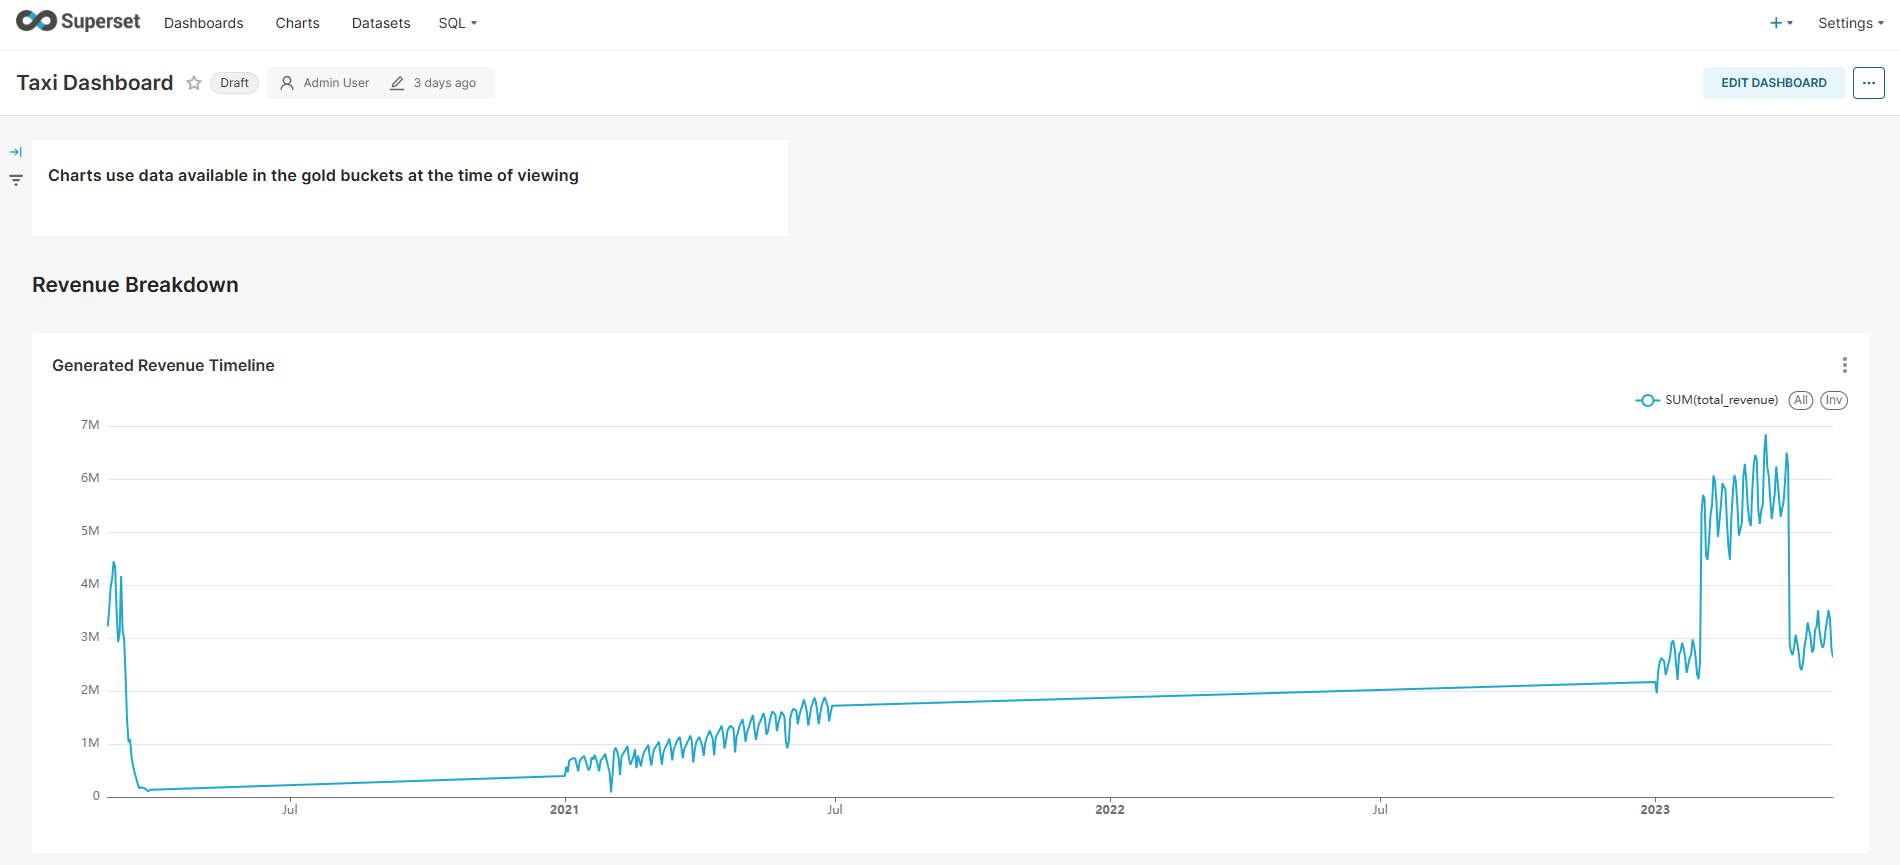
\includegraphics[width=\textwidth]{taxi_dashboard.png}
    \caption{TLC Yellow Trip Dashboard}
    \label{fig:dashboardtaxi}
\end{figure*}

%% Weather Dashboard Diagram
\begin{figure*}[t]
    \centering
    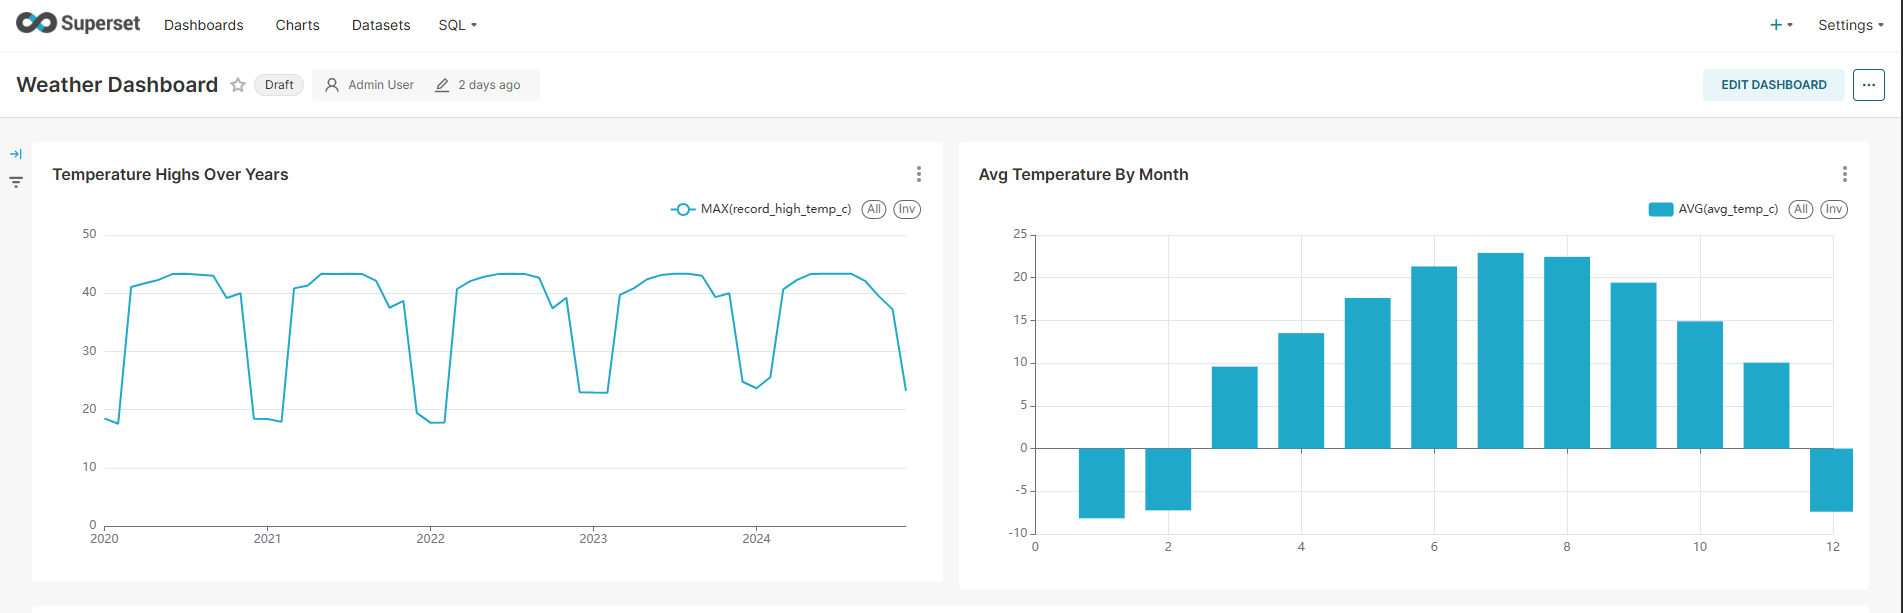
\includegraphics[width=\textwidth]{weather_dashboard.png}
    \caption{NOAA GSOD Dashboard}
    \label{fig:dashboardweather}
\end{figure*}

\subsubsection{Dashboard Visualization}
From observing the dashboard configured to visually validate the usefulness of the Gold aggregated data generated, we observe that all data generated is reasonable with no invalid values being displayed which confirms that cleaning and aggregation was successful in the pipeline. Graphs were correctly generated for the two datasets with Figure~\ref{fig:dashboardtaxi} showing a sample line graph for revenue generated over the years for the TLC Yellow Trip data on the Taxi dashboard. Figure~\ref{fig:dashboardweather} also demonstrates that the NOAA GSOD dataset had its data correctly aggregated with a reasonable bar chart and line graph being created for the dataset.

%% Taxi Dashboard Diagram
\begin{figure*}[t]
    \centering
    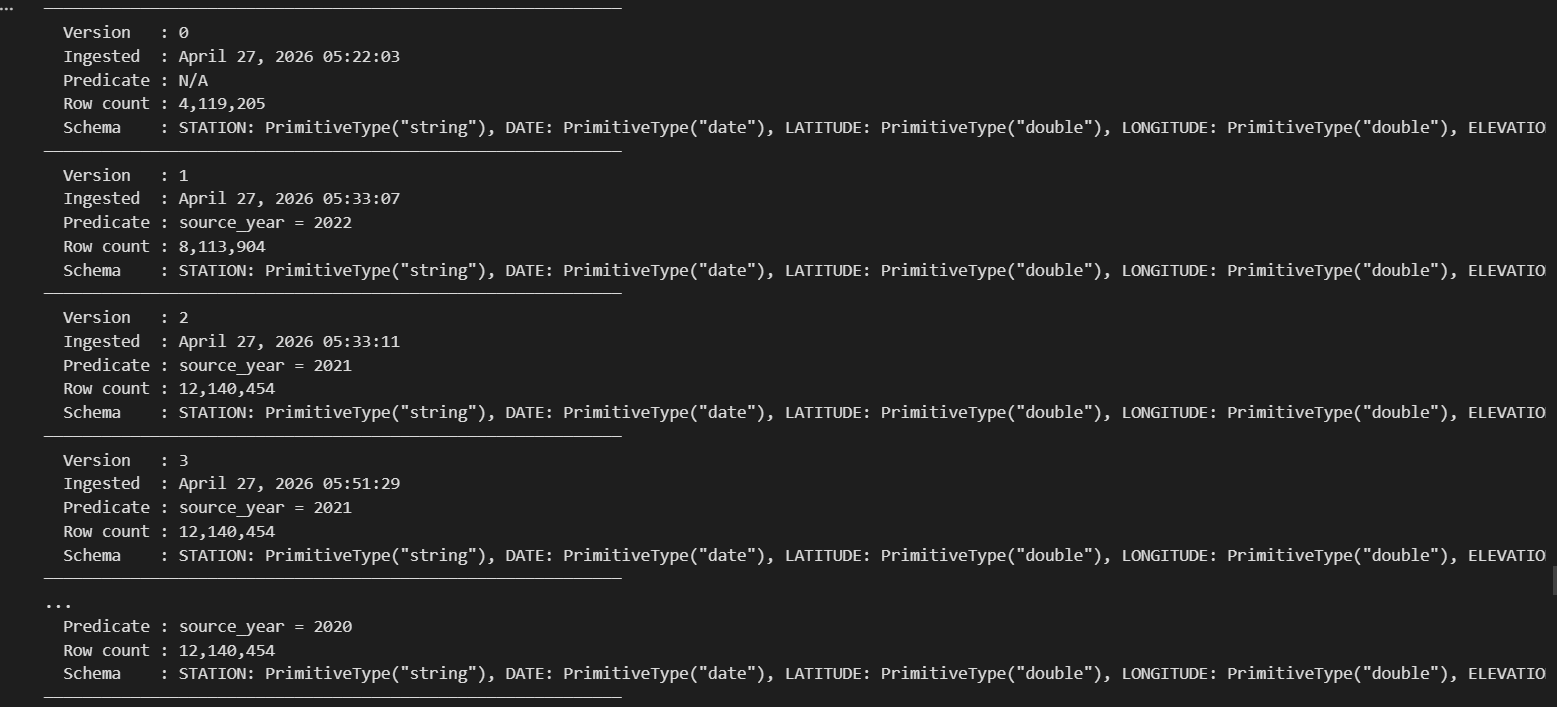
\includegraphics[width=\textwidth]{weather_time_travel.png}
    \caption{TLC Yellow Trip Dashboard}
    \label{fig:dashboardtaxi}
\end{figure*}

\subsubsection{Time Travel Queries}
Time travel queries were also successfully implemented with the recent versions of files in each bucket being able to be retrieved. The versions also showed which date the files were ingested into the Delta Table for that bucket and what operations were performed on them. Furthermore, we are also given insight into the number of rows present in the bucket for each version with Figure~\ref{fig:timetravelbronzeweather} showing the number of rows and the date ingested for the first 5 versions of the Bronze bucket of the NOAA GSOD data. This same output is possible for all 3 layers for both datasets along with the schema being shown at each step. This will be useful for auditing both datasets and for schema enforcement.

\subsection{Limitations}
The proposed design has a few limitations with some being development limitations only. They are as follows:
\begin{enumerate}
    \item \textbf{DuckDB can not read/write Delta Tables.} This may have been a limitation with version 1.4.4 of DuckDB being used with deltalake 1.5.0. Upon further investigation it was found that DuckDB has trouble setting S3 credentials when reading/writing Delta tables to MinIO with the underlying problem stemming from the Rust kernel of delta-rs. The workaround to this was using Pyarrow for Delta table read/writes however using DuckDB alone would save the in-memory cost of storing the data as an arrow table.
    \item \textbf{Limited compute power} The machine used for testing was able to process rows of 2-6M comfortably however beyond this limit the machine could not handle processing of the data without crashing or timing out.
    \item \textbf{No streaming ingestion} Streaming ingestion was not implemented for this pipeline despite it being more optimal for the proposed pipeline. Apache Kafka could be used to implement streaming ingestion in the future and further optimize the pipeline
    \item \textbf{Schema evolution does not handle column name case changes} The current implementation does not gracefully handle column case changes with new columns being created all together. This can fully break the pipeline where it is not handled in this implementation and could be handled through converting all column names in both datasets to either lower or uppercase at the Bronze Ingest before any further processing is done.
\end{enumerate}

\section{Conclusions and Insights}
\label{sec:conclusion}

A lightweight Data Lakehouse solution was achieved using MinIO and DuckDB as our main storage service and query engine respectfully with a reliable data pipeline being developed where schema evolution was handled and queries were optimized for one node. The main takeaways from this were: 

\begin{enumerate}
    \item \textbf{Schema evolution handled} The current solutions gracefully handles schema evolution in the case of column additions and deletions to the dataset. When new columns are added the schema is simply merged with the existing one in the database while if a required column is removed, the data is not ingested all together and the pipeline stops processing.
    \item \textbf{Data successfully processed and stored at 3 layers} Both datasets had its data stored from 2019 onward successfully with each layer catering to different use cases all together. Machine Learning could be done using data the Silver layer while business analytics could be gained from the Gold layer with dashboards being developed as demonstrated.
    \item \textbf{Pipeline optimized for single node} The current solution runs gracefully on a single node with just DuckDB and MinIO with there being no noticeable crashes, slow downs or errors in the data at any layer. This proves that a distributed system is not always required for efficient Data Lakehouse implementations.
\end{enumerate}

\section{Reflection on Project Process and Challenges}
\label{sec:reflection}

Work was divided equally among the two members who worked on this project. Arvesh handled the main architectural conception, docker development environment setup and had major contributions to both pipelines at each step. Nie-l helped polish the implementation of both pipelines, notably at the Gold Transform step where most aggregations were devised by him. Nie-l also helped in creating additional validation checks for both datasets to ensure a reliable pipeline was delivered.

Three challenges are worth naming:
\begin{itemize}
    \item \textbf{Limited compute power in development} The 2019 dataset for the TLC Yellow Trip data was notably large with there being 7M+ records per month. This led to our pipeline often crashing at the Silver Transforms or Silver Validation stages of our pipeline as the workload became too much for the development machine to handle.
    \item \textbf{NOAA GSOD being very unreliable} Given the nature of instruments used for measuring weather related metrics, the dataset is expected to have many unreliable figures however this made development of validation suites for the NOAA GSOD dataset very difficult with majority of the dataset needing to be dropped at times (1-2M+ records).
    \item \textbf{Unpredictable dataset release dates} The current orchestration gives a few days grace period before trying to ingest data for a new month/year for both datasets however in reality there is no way of reliably knowing when the dataset will be released. This could reliably solved with sensors in Apache Airflow in other iteration of this project.
\end{itemize}

Contributions were tracked in a shared board and validated in the individual interviews. We used AI tools (Claude and Copilot) for drafting documentation, generating unit-test skeletons, and clarifying Spark error messages. All modeling decisions, feature choices, and final analysis were made by the authors.

\section{Quality of Code and Reproducibility}
\label{sec:code}

The source repository is organized into \texttt{ingestion/} (ingestion for Bronze and Gold along with raw download scripts), \texttt{notebooks/} (query performance analysis and time travel query demonstration), \texttt{dashboard/} (the sample Superset + Trino dashboard developed), \texttt{quality/} (the validation suites for Bronze and Silver), \texttt{transformations/} (the Silver and Gold transformations where Gold transformations are found in the dbt project in \texttt{dbt/}) and \texttt{docs/}. Dependencies are pinned in \texttt{requirements.txt}; a Docker Compose file brings up MinIO, Apache Airflow, Superset, Trino, a postgres databse for Trino metadata, various init commands for services and a dbt API. By using the Apache Airflow Web UI hosted at port 8080 locally, the pipeline can be ran for both the Taxi and Weather datasets. Port 9001 then hosts MinIO GUI where you can visually see the data stored, port 8088 hosts the dashboard for viewing the analytical Gold data and port 8001 hosts the dbt API.

\section*{Acknowledgements}
We thank Mr.\ Sergio Mathurin and Mr.\ Anton Greenridge for guidance throughout the course and the great deal of help given to us during the development at this project with Mr.\ Anton Greenridge being very patient in guiding us through each stage of our Lakehouse design, and the NYC TLC along with NOAA for making their trip-level data publicly available.

\begin{thebibliography}{00}
\bibitem{tlc} NYC Taxi and Limousine Commission, ``TLC Trip Record Data,'' 2024. [Online]. Available: \url{https://www.nyc.gov/site/tlc/about/tlc-trip-record-data.page}
\bibitem{noaa} National Oceanic and Atmospheric Administration, ``Global Surface Summary of the Day (GSOD),'' 2024. [Online]. Available: \url{https://www.ncei.noaa.gov/products/land-based-station/global-surface-summary-of-day}
\bibitem{armbrust2021lakehouse} M. Armbrust, A. Ghodsi, R. Xin, and M. Zaharia, ``Lakehouse: A New Generation of Open Platforms that Unify Data Warehousing and Advanced Analytics,'' in \textit{Proc. 11th Conf. on Innovative Data Systems Research (CIDR)}, 2021.
\bibitem{armbrust2020deltalake} M. Armbrust, T. Das, L. Sun, et al., ``Delta Lake: High-Performance ACID Table Storage over Cloud Object Stores,'' \textit{Proc. VLDB Endowment}, vol. 13, no. 12, pp. 3411--3424, 2020.
\bibitem{databricks_medallion} Databricks, ``What is the Medallion Lakehouse Architecture?'' 2023. [Online]. Available: \url{https://docs.databricks.com/lakehouse/medallion.html}
\bibitem{raasveldt2019duckdb} M. Raasveldt and H. M\"{u}hleisen, ``DuckDB: An Embeddable Analytical Database,'' in \textit{Proc. 2019 ACM SIGMOD Int. Conf. on Management of Data}, pp. 1981--1984, 2019.
\bibitem{ge_docs} Great Expectations, ``GX Core: Open Source Data Quality Platform,'' 2024. [Online]. Available: \url{https://greatexpectations.io/gx-core/}
\bibitem{airflow_docs} Apache Software Foundation, ``Apache Airflow Documentation,'' 2024. [Online]. Available: \url{https://airflow.apache.org/docs/}
\bibitem{dbt_docs} dbt Labs, ``What is dbt?'' 2024. [Online]. Available: \url{https://docs.getdbt.com/docs/introduction}
\bibitem{minio_docs} MinIO, ``MinIO High Performance Object Storage,'' 2024. [Online]. Available: \url{https://min.io/docs/minio/linux/index.html}
\bibitem{fastapi_docs} S. Ramirez, ``FastAPI Documentation,'' 2024. [Online]. Available: \url{https://fastapi.tiangolo.com}
\bibitem{superset_docs} Apache Software Foundation, ``Apache Superset Documentation,'' 2024. [Online]. Available: \url{https://superset.apache.org/docs/intro}
\bibitem{pyarrow_docs} Apache Software Foundation, ``Apache Arrow and PyArrow Documentation,'' 2024. [Online]. Available: \url{https://arrow.apache.org/docs/python/}
\bibitem{trino_docs} Trino Software Foundation, ``Trino Documentation,'' 2024. [Online]. Available: \url{https://trino.io/docs/current/}
\end{thebibliography}

\appendix
\section*{AI Tools Used}
The main tool used in this project was Claude with it giving us (i) tutorials and articles on setting up the development environment, (ii) syntax for achieving the desired outputs of our solutions, (iii) architectural guidance in what technologies work the best and the pros and cons of each, (iv) formatting guidance in generating this report and (v) explanations on various Lakehouse concepts required to develop this project.

\end{document}
